\documentclass{article}
\usepackage[vmargin={15mm}, hmargin={30mm}]{geometry}
\usepackage{amsmath}
\usepackage{graphicx}
\usepackage[utf8]{inputenc}
\usepackage[english]{babel}
\usepackage[]{amsthm} %lets us use \begin{proof}
\usepackage[]{amssymb} %gives us the character \varnothing

\title{IL2230 HADL \\ Lab1: Handwritten Digits Recognition from MLP to CNN}
\author{Irene, Zhao Linghan, Wang Jiayang, Tu Han}
%This information doesn't actually show up on your document unless you use the maketitle command below

\begin{document}
\maketitle %This command prints the title based on information entered above

%Section and subsection automatically number unless you put the asterisk next to them.
\section*{Part 1: CNN in Pytorch}
\subsection*{1.1 Variance in accuracy based on the number of features maps in layer 1 and 2.}
To study the variance in accuracy in the CNN we create a Python code that iterates through the different values that we want to test in each convolutional layer. In order to achieve the best possible results we have studied which number of epoch is optimal to use for the training, as we can see in the following graph: \\
\begin{figure}[h]
    \centering
    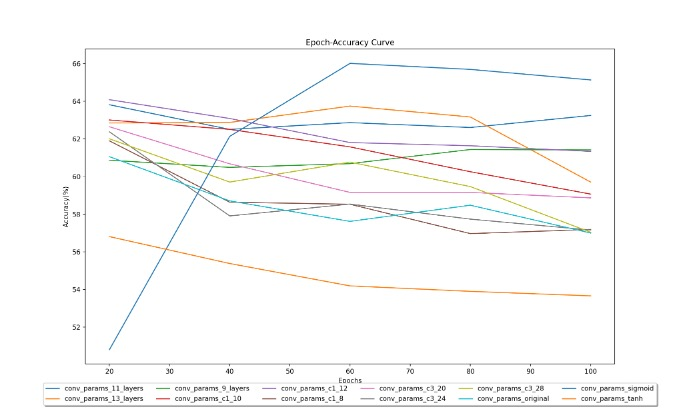
\includegraphics[width=15cm]{Epoch_Accuracy.jpg}
    \label{fig:my_label}
\end{figure}
\subsection*{1.2 Variance in accuracy based on the number of layers in the network.}

\subsection*{1.3 Variance in accuracy based on type of activation layer.}

\section*{Part 2: Handwritten Digits Recognition}
\subsection*{2.1 Variance in accuracy based on number of neurons for layers 1 and 2.}
\subsection*{2.2 Practical information and comparison using pytorch profiler.}
\end{document}